\begin{apendicesenv}

\partapendices

\chapter{Grafos}

\section{Um Pouco mais de História}

Graças à resolução dada por Euler, mais tarde muitos outros problemas importantes, para o desenvolvimento da Matemática Aplicada, foram possíveis de serem modelados. Um desses modelos são as relações de amizade, de hierarquia, de trabalho. Netto \cite{Netto:2012}, aponta grafos como um auxílio para o estudo de problemas envolvendo inter-relacionamento de elementos (em química orgânica, eletricidade, organização, transporte, psicossociologia). Na verdade, grafos modelam diversas situações e muitas delas não quantificáveis.

Conforme Ore \cite{Ore:1963}, no século seguinte, o matemático irlandês William Hamilton, em 1859, inventou um jogo chamado ``\textit{The Icosian Game}'', com um peculiar enigma envolvendo um dodecaedro, em que cada um dos 20 vértices foram nomeados com nomes de cidades importantes. O objetivo do jogo era, utilizando as 30 arestas do dodecaedro, passar por cada uma das cidades apenas uma vez, começando e terminando na mesma cidade. Um exemplo do grafo pode ser visualizado na Figura \ref{grafo_hamiltoniano}.

\begin{figure}[!h]
	\centering
	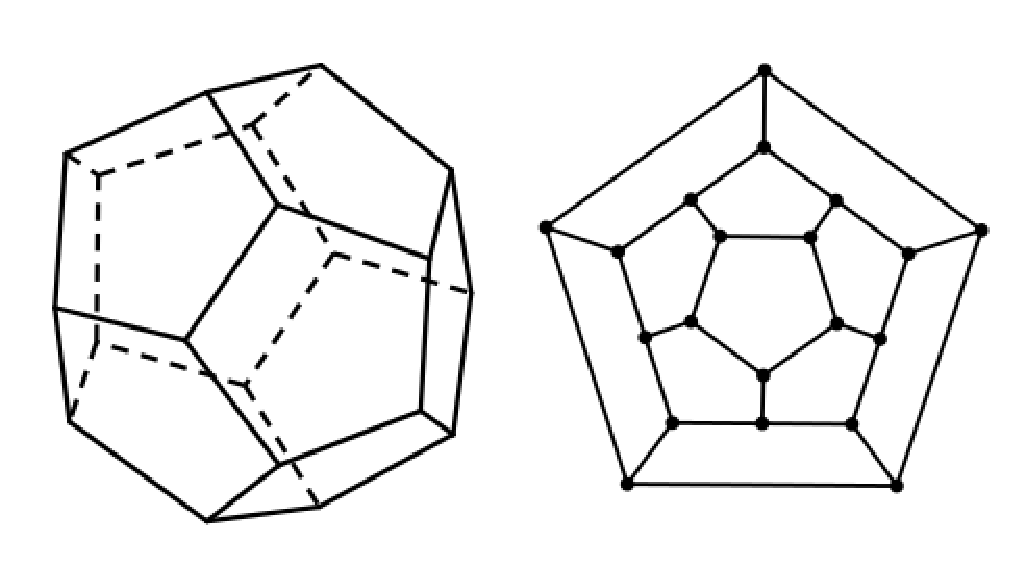
\includegraphics[scale=0.3]{figuras/capitulo2/grafo_hamiltoniano.eps}
	\caption[Grafo hamiltoniano]{Grafo hamiltoniano \cite{Ore:1963}}
	\label{grafo_hamiltoniano}
\end{figure}

Apesar da simples formulação, o problema admite muitos caminhos como resposta. No problema de Hamilton, temos uma diferença significativa em relação ao problema de Euler. Encontrar um caminho euleriano significa encontrar um caminho que passe por todas as arestas do grafo uma única vez, podendo ser aberto ou fechado. Nos caminhos hamiltonianos, cada vértice é visitado uma única vez. O problema fica mais complexo com tal condição \cite{Costa:2011}.

\section{Outras Definições}

Um grafo é finito se tanto o seu conjunto de vértices, quanto o seu conjunto de arestas são finitos. Um grafo sem vértices (e, portanto, sem arestas) é o grafo nulo. Qualquer grafo apenas com um vértice é referido como trivial. Todos os outros grafos são não-triviais \cite{Costa:2011}.

Um grafo é simples se não tem \textit{loops} ou arestas paralelas \cite{Diestel:1997}, como exemplificado na Figura \ref{grafo_simples}.

\begin{figure}[!h]
	\centering
	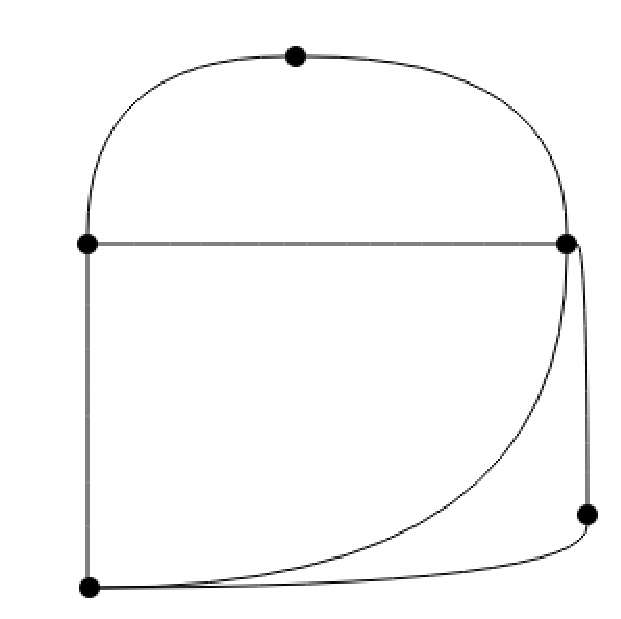
\includegraphics[scale=0.2]{figuras/capitulo2/grafo_simples.eps}
	\caption[Exemplo de grafo simples]{Exemplo de grafo simples \cite{Costa:2011}}
	\label{grafo_simples}
\end{figure}

Certos tipos de grafos podem desempenhar papéis proeminentes na teoria dos grafos. Um grafo conexo é um grafo simples no qual quaisquer dois vértices são ligados por um caminho. Um grafo é vazio quando não há dois vértices adjacentes (isto é, o conjunto de arestas é vazio). Um grafo é bipartido se o seu conjunto de vértices pode ser particionado em dois subconjuntos \textit{X} e \textit{Y} para que cada aresta tem um fim em \textit{X} e um fim em \textit{Y}; uma tal partição (\textit{X}, \textit{Y}) é chamada uma bipartição do grafo, e \textit{X} e \textit{Y} suas partes. Pode-se denotar um grafo bipartido \textit{G} com bipartição (\textit{X}, \textit{Y}) por \textit{G}[\textit{X}, \textit{Y}]. Se \textit{G}[\textit{X}, \textit{Y}] é simples e todos os vértices de \textit{X} estão associados a cada vértice em \textit{Y}, então \textit{G} é chamado de um grafo bipartido completo. Uma estrela é um grafo bipartido completo \textit{G}[\textit{X}, \textit{Y}] com |\textit{X}| = 1 ou |\textit{Y}| = 1 \cite{Diestel:1997}.  A Figura \ref{tipos_grafos} ilustra estes tipos de grafos, sendo o grafo ``A'' é um grafo conexo, o grafo ``B'' é um grafo vazio e o grafo ``C'' é um grafo bipartido completo.

\begin{figure}[!h]
	\centering
	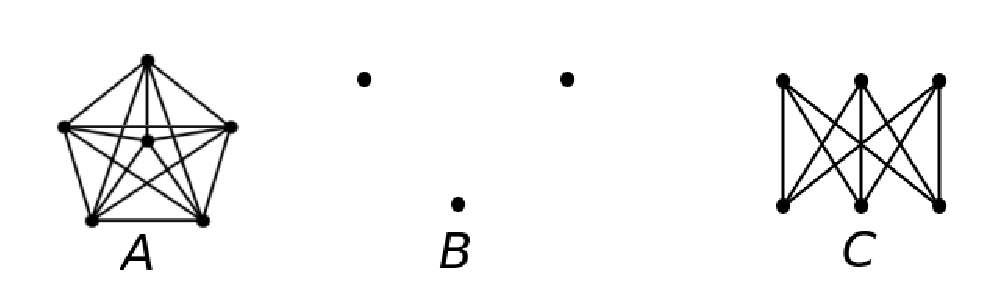
\includegraphics[scale=0.4]{figuras/capitulo2/tipos_grafos.eps}
	\caption[Tipos de grafos]{Tipos de grafos \cite{Diestel:1997}}
	\label{tipos_grafos}
\end{figure}

Um caminho é um grafo simples cujos vértices podem ser dispostos em uma sequência linear. De tal forma que dois vértices são adjacentes se forem consecutivos na sequência, e não adjacentes caso não forem consecutivos \cite{Bondy:2007}. Dessa forma, diz-se que um vértice é alcançável a partir de outro, se houver um caminho levando o primeiro vértice ao último \cite{Costa:2011}. A Figura \ref{caminho} apresenta um caminho (arestas em vermelho) do vértice ``a'' até o vértice ``e''.

\begin{figure}[!h]
	\centering
	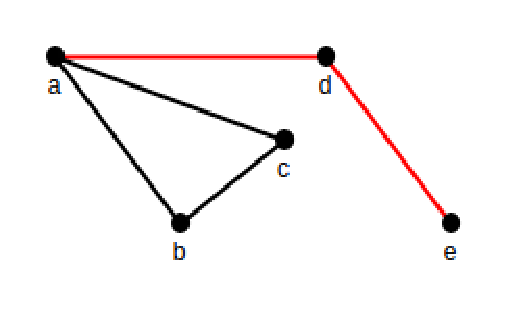
\includegraphics[scale=0.5]{figuras/capitulo2/caminho.eps}
	\caption[Caminho]{Caminho \cite{Costa:2011}}
	\label{caminho}
\end{figure}

Do mesmo modo, um ciclo é um grafo simples cujos vértices podem ser dispostos em uma sequência cíclica de tal maneira que dois vértices são adjacentes se forem consecutivos na sequência. O comprimento de um caminho ou de um ciclo é o número de suas arestas \cite{Costa:2011}. É possível observar na Figura \ref{ciclos} alguns exemplos de grafos com ciclo.

\begin{figure}[!h]
	\centering
	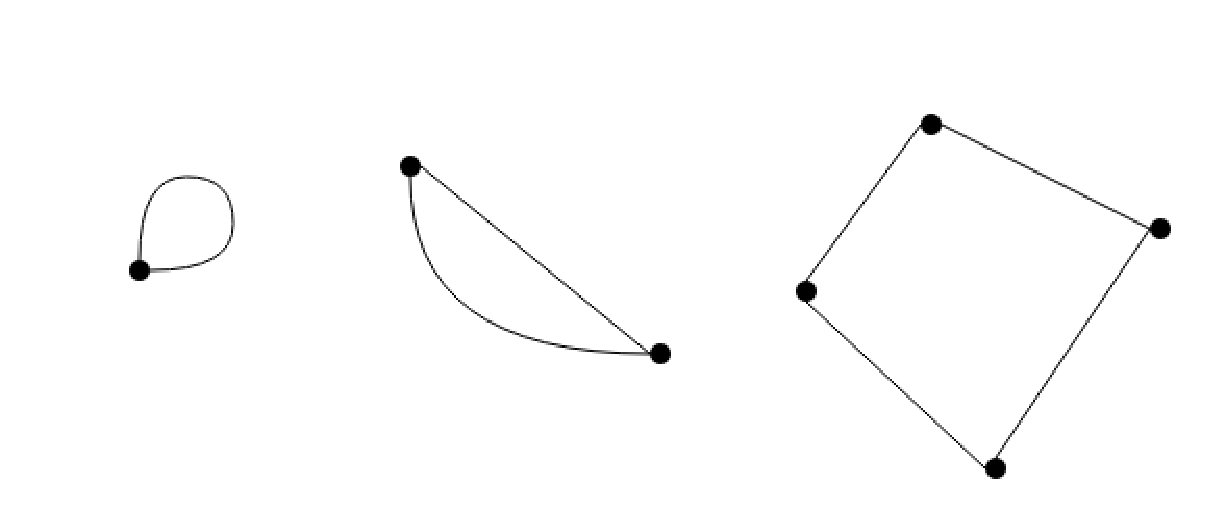
\includegraphics[scale=0.3]{figuras/capitulo2/ciclos.eps}
	\caption[Exemplo de grafos com ciclos]{Exemplo de grafos com ciclos \cite{Costa:2011}}
	\label{ciclos}
\end{figure}

Um grafo é conectado se, para cada partição de seus vértices definido em dois conjuntos \textit{X} e \textit{Y} não vazios, existe uma aresta com uma extremidade em \textit{X} e uma extremidade em \textit{Y}; caso contrário, o grafo é desconectado. Em outras palavras, um grafo é desconectado se o conjunto de vértices pode ser particionado em dois subconjuntos não vazios \textit{X} e \textit{Y} e que nenhuma aresta tem uma extremidade em \textit{X} e a outra extremidade em \textit{Y}. É instrutivo comparar esta definição com a de um grafo bipartido. Os exemplos de grafos conectados e desconectados são apresentados na Figura \ref{desconectados}, onde o grafo ``X'' e o grafo ``Y'' são dois grafos distintos conectados. Porém se fossem trados como um único grafo, este seria um grafo desconectado \cite{Bondy:2007}.

\begin{figure}[!h]
	\centering
	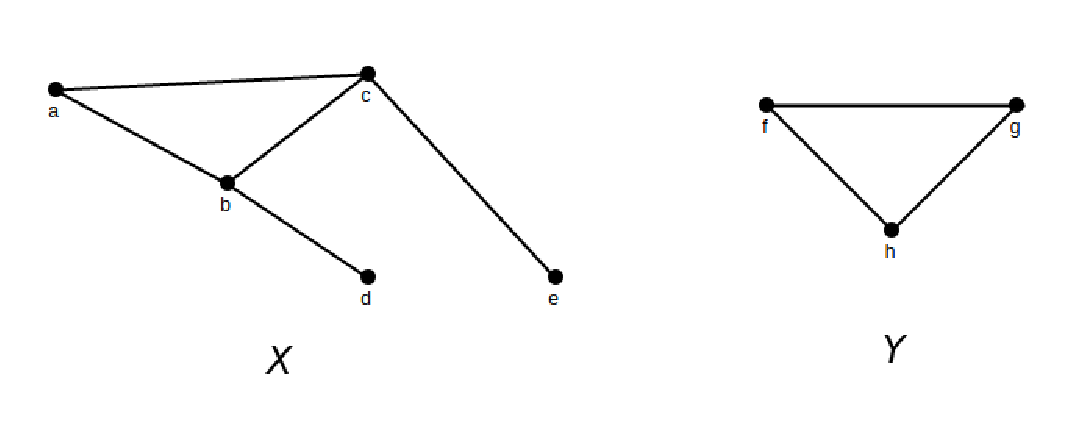
\includegraphics[scale=0.45]{figuras/capitulo2/desconectados.eps}
	\caption[Exemplo de grafos conectados e desconectados]{Exemplo de grafos conectados e desconectados \cite{Bondy:2007}}
	\label{desconectados}
\end{figure}

O grau de um vértice \textit{v} em um grafo \textit{G}, designado por \textit{d$_G$}(\textit{v}), é o número de arestas de \textit{G} que incidem em \textit{v}; para cada \textit{loop} é contado duas arestas. Em particular, se \textit{G} é um grafo simples, \textit{d$_G$}(\textit{v}) é o número de vizinhos de \textit{v} em \textit{G}. Um vértice de grau zero é chamado um vértice isolado. Denominamos por $\delta$(\textit{G}) e $\Delta$(\textit{G}) mínimo e máximo graus dos vértices de \textit{G}, e por \textit{d}(\textit{G}), o seu grau médio, $\frac{1}{n}\sum_{\textit{v}\in\textit{V}} \textit{d}(\textit{v})$ \cite{Diestel:1997}.

\section{Árvores e Florestas}

Um grafo acíclico é aquele que não contém ciclos. Um grafo acíclico conectado é chamado de uma árvore. As árvores com seis vértices estão apresentadas na Figura \ref{arvores_seis_vertices}. De acordo com estas definições, cada componente de um grafo acíclico é uma árvore. Por esta razão, grafos acíclicos são geralmente chamados florestas \cite{Bondy:2007}.

\begin{figure}[!h]
	\centering
	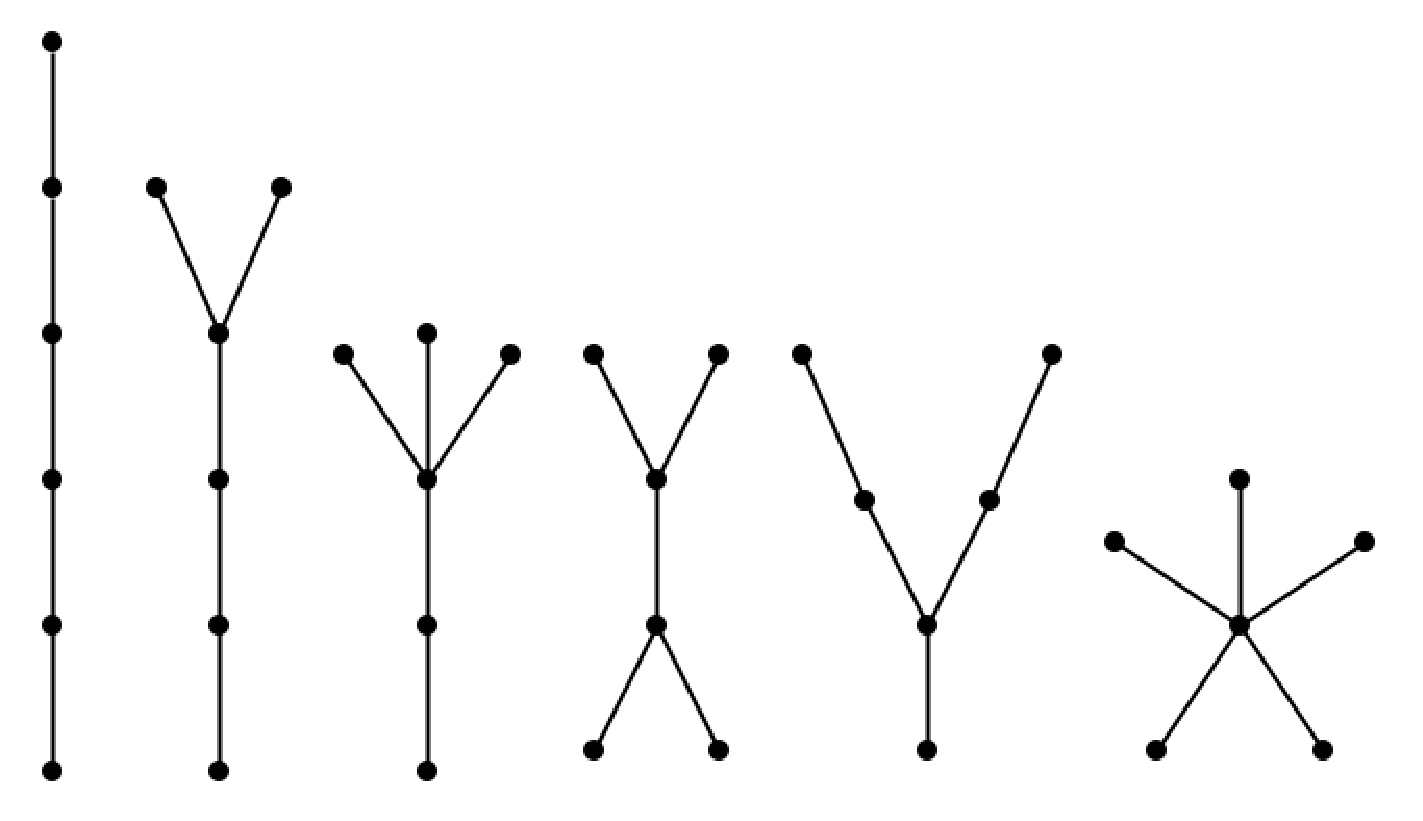
\includegraphics[scale=0.2]{figuras/capitulo2/arvores_seis_vertices.eps}
	\caption[Exemplo de árvores com seis vértices]{Exemplo de árvores com seis vértices \cite{Bondy:2007}}
	\label{arvores_seis_vertices}
\end{figure}

Em uma árvore, quaisquer dois vértices são conectados por exatamente um caminho. E Diestel \cite{Diestel:1997} representa esse único caminho de ligação vértices \textit{x} e \textit{y} em uma árvore \textit{T} por \textit{xTy}.

Uma árvore com raiz \textit{T}(\textit{x}) é uma árvore \textit{T} com um vértice específico \textit{x}, chamado a raiz de \textit{T}. Em uma orientação de uma árvore com raiz, todos vértices, excluindo o vértice raiz \textit{x}, é chamado de ramificação \cite{Bondy:2007}. Um exemplo de uma árvore com raiz pode ser observado na Figura \ref{arvore_raiz}.

\begin{figure}[!h]
	\centering
	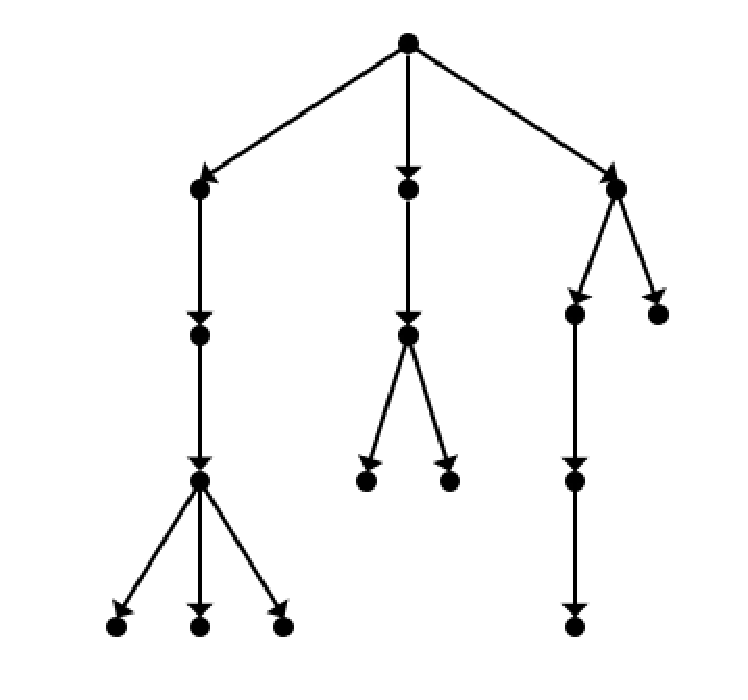
\includegraphics[scale=0.2]{figuras/capitulo2/arvore_raiz.eps}
	\caption[Exemplo de uma árvore com raiz]{Exemplo de uma árvore com raiz \cite{Bondy:2007}}
	\label{arvore_raiz}
\end{figure}

\chapter{Algoritmos}

\section{Exemplificação DFS}
\label{sec:exemplificacao dfs}

Considere as Figuras a seguir para a exemplificação do DFS.

\begin{figure}[!h]
	\centering
	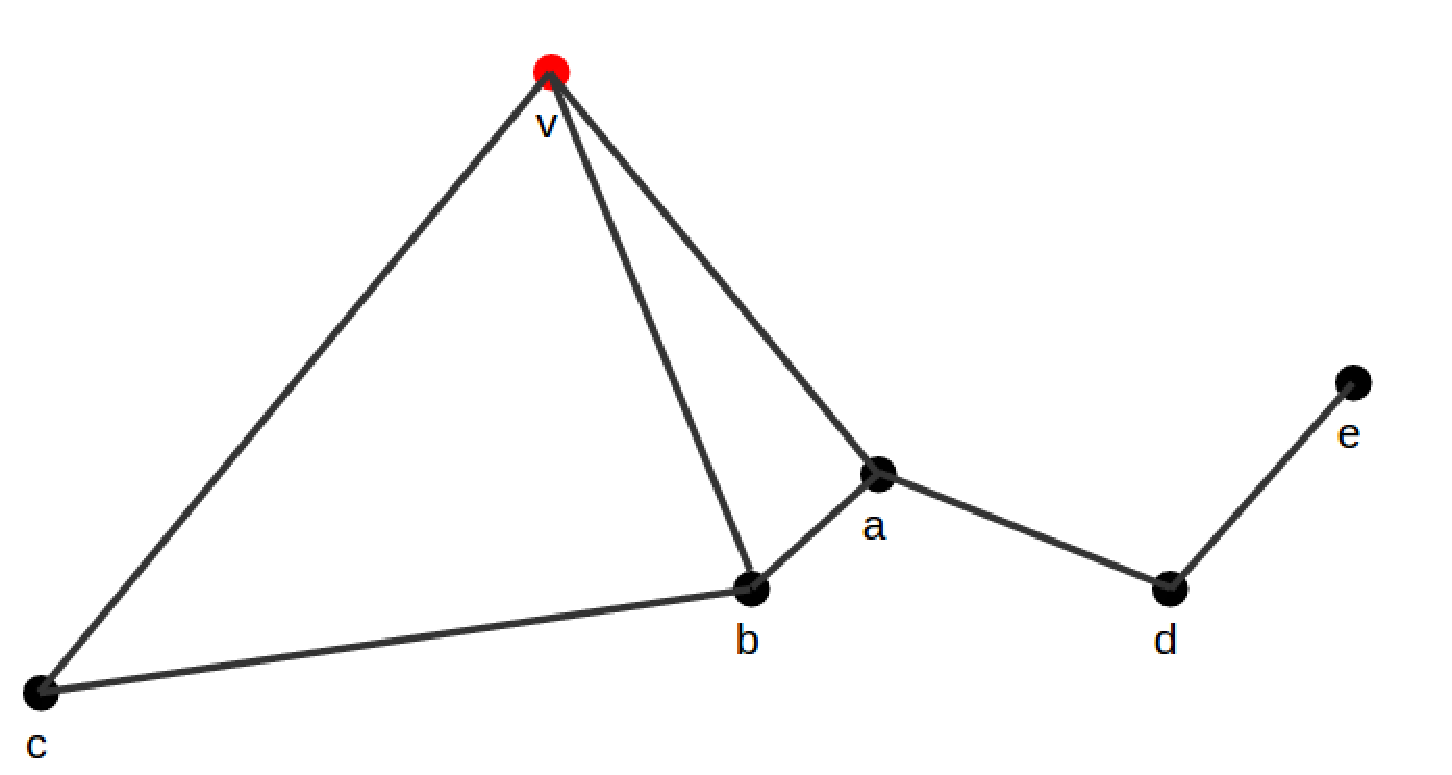
\includegraphics[scale=0.25]{figuras/capitulo2/dfs/dfs1.eps}
	\caption[Exemplo DFS etapa 1]{Exemplo DFS etapa 1 \cite{Cormen:2001}}
	\label{dfs1}
\end{figure}

A busca irá partir do vértice arbitrário \textit{v}, chamado de vértice raiz. A partir do vértice raiz é possível percorrer três arestas: (\textit{v}, \textit{a}), (\textit{v}, \textit{b}) e (\textit{v}, \textit{c}). A aresta a ser seguida será (\textit{v}, \textit{a}).

\begin{figure}[!h]
	\centering
	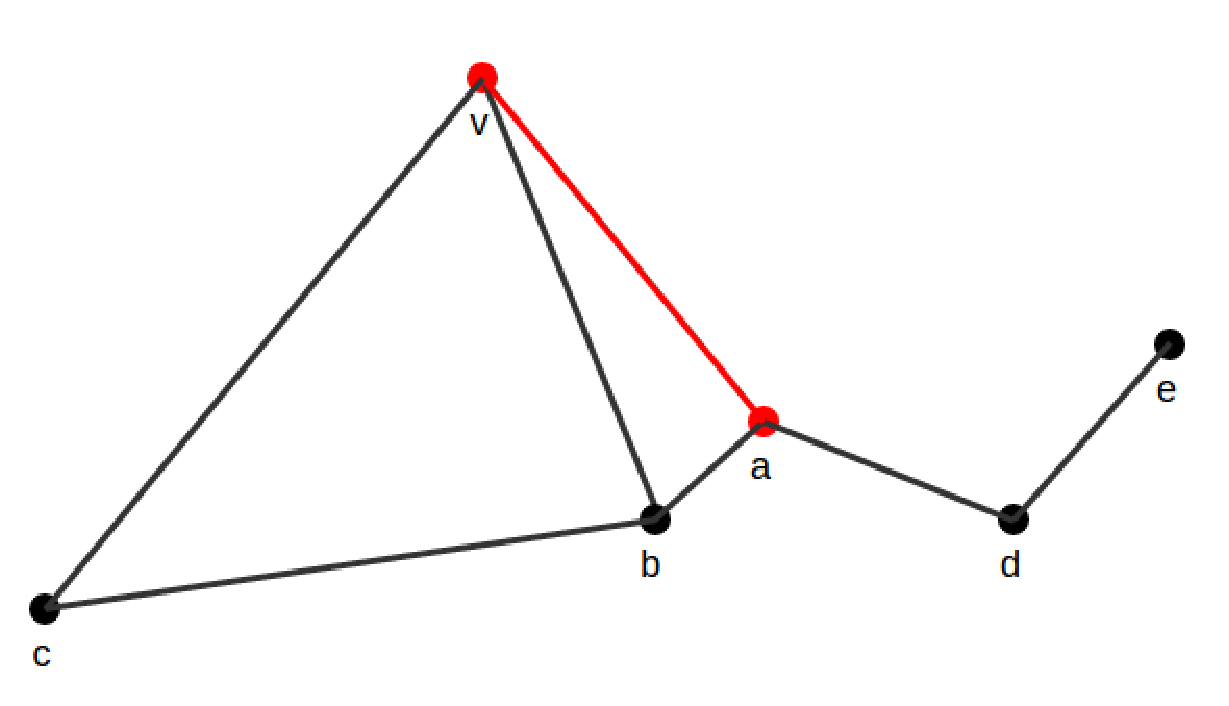
\includegraphics[scale=0.25]{figuras/capitulo2/dfs/dfs2.eps}
	\caption[Exemplo DFS etapa 2]{Exemplo DFS etapa 2 \cite{Cormen:2001}}
	\label{dfs2}
\end{figure}

O vértice \textit{a} possui três arestas, que são: (\textit{a}, \textit{v}), (\textit{a}, \textit{b}) e (\textit{a}, \textit{d}). Como o vértice \textit{v} já foi visitado, a aresta a ser seguida será (\textit{a}, \textit{b}).

\begin{figure}[!h]
	\centering
	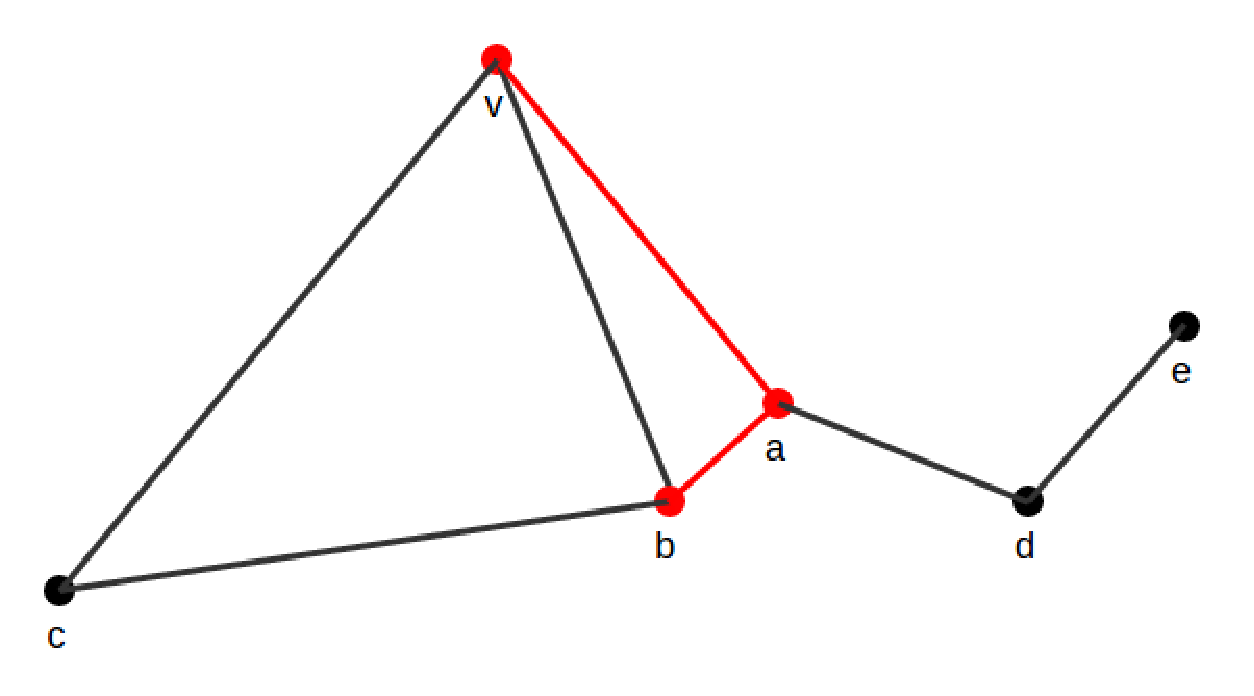
\includegraphics[scale=0.25]{figuras/capitulo2/dfs/dfs3.eps}
	\caption[Exemplo DFS etapa 3]{Exemplo DFS etapa 3 \cite{Cormen:2001}}
	\label{dfs3}
\end{figure}

A partir de \textit{b}, é possível escolher as seguintes arestas: (\textit{b}, \textit{v}), (\textit{b}, \textit{a}) e (\textit{b}, \textit{c}). Porém como os vértices \textit{v} e \textit{a} já foram visitados, a opção restante será a aresta (\textit{b}, \textit{c}).

\newpage

\begin{figure}[!h]
	\centering
	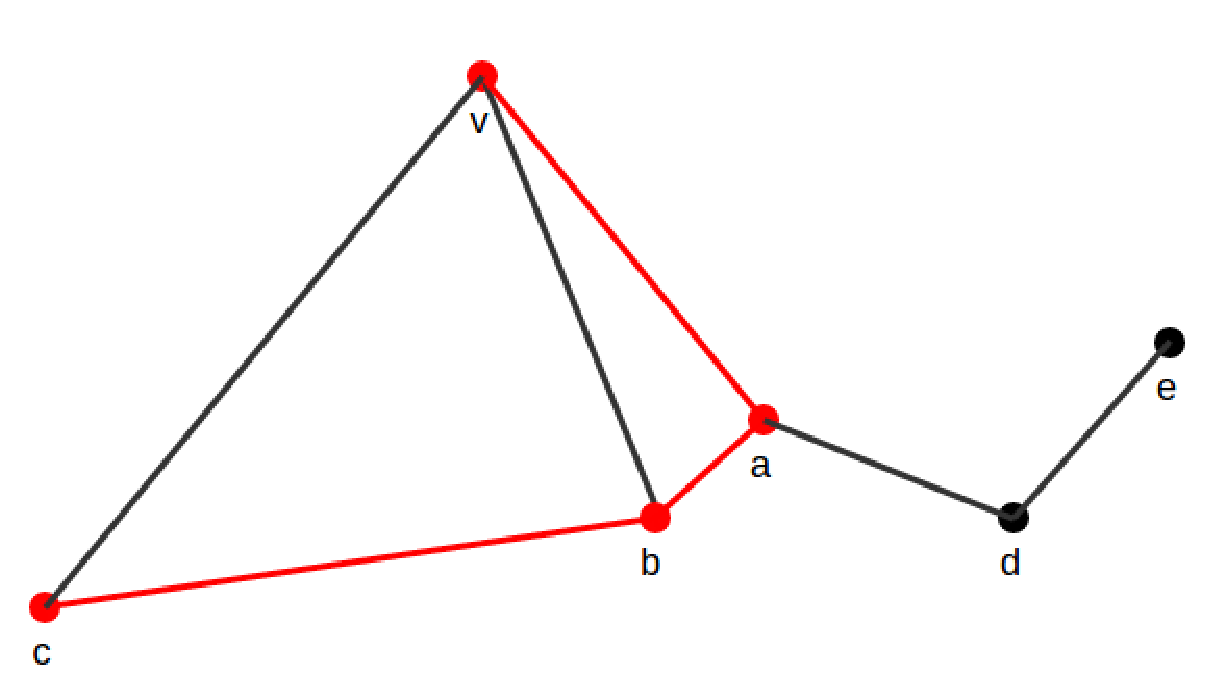
\includegraphics[scale=0.25]{figuras/capitulo2/dfs/dfs4.eps}
	\caption[Exemplo DFS etapa 4]{Exemplo DFS etapa 4 \cite{Cormen:2001}}
	\label{dfs4}
\end{figure}

Ao alcançar \textit{c}, há duas possibilidades: (\textit{c}, \textit{v}) e (\textit{c}, \textit{b}). Porém ambos os vértices \textit{v} e \textit{b} já são conhecidos. Neste caso não há para onde se aprofundar. Entretanto, ainda existem vértices não descobertos. Nesse caso, deve-se voltar até o vértice \textit{b}, verificando se há alguma aresta que leva a um vértice ainda não visitado. Caso ocorra tal situação, deve-se voltar novamente pelo caminho percorrido, chegando ao vértice \textit{a}. Em \textit{a}, a aresta (\textit{a}, \textit{d}) leva a um vértice ainda não descoberto, portanto, esse caminho deve ser tomado.

\begin{figure}[!h]
	\centering
	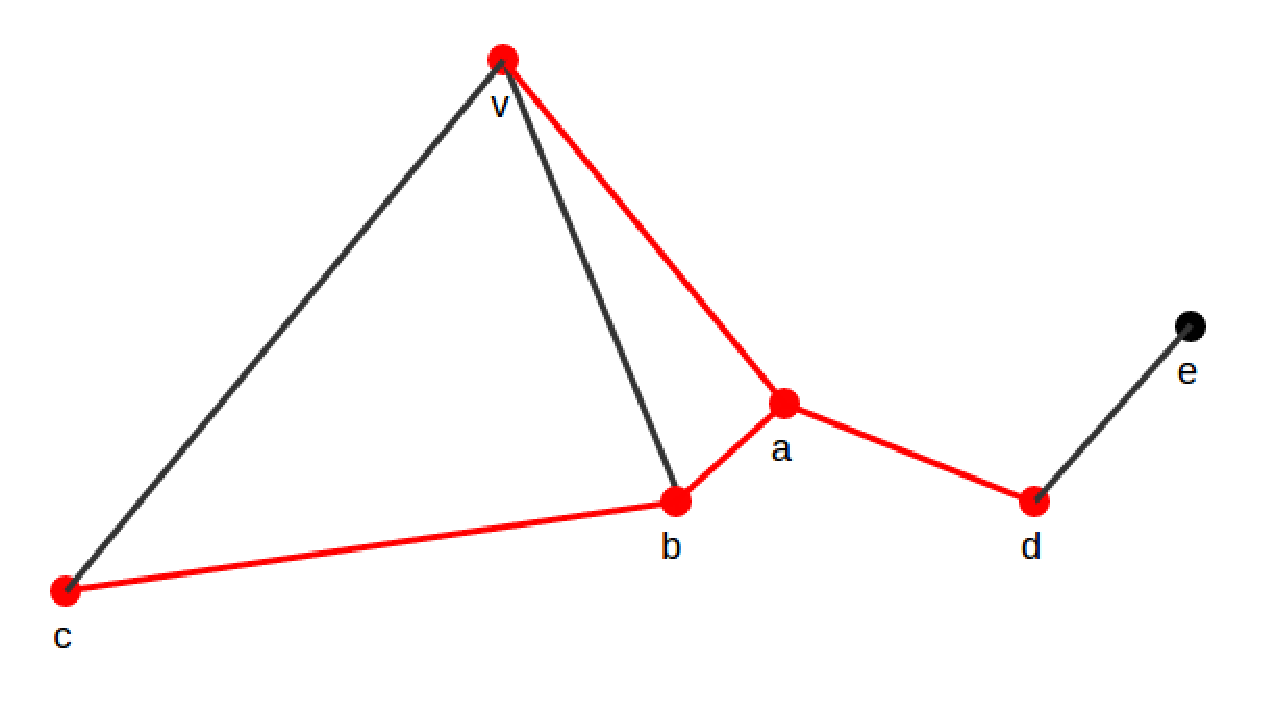
\includegraphics[scale=0.25]{figuras/capitulo2/dfs/dfs5.eps}
	\caption[Exemplo DFS etapa 5]{Exemplo DFS etapa 5 \cite{Cormen:2001}}
	\label{dfs5}
\end{figure}

Em \textit{d}, há dois caminhos a seguir: (\textit{d}, \textit{a}) e (\textit{d}, \textit{e}). Porém a única aresta que leva a um vértice não visitado é (\textit{d}, \textit{e}). Esta deverá ser seguida.

\begin{figure}[!h]
	\centering
	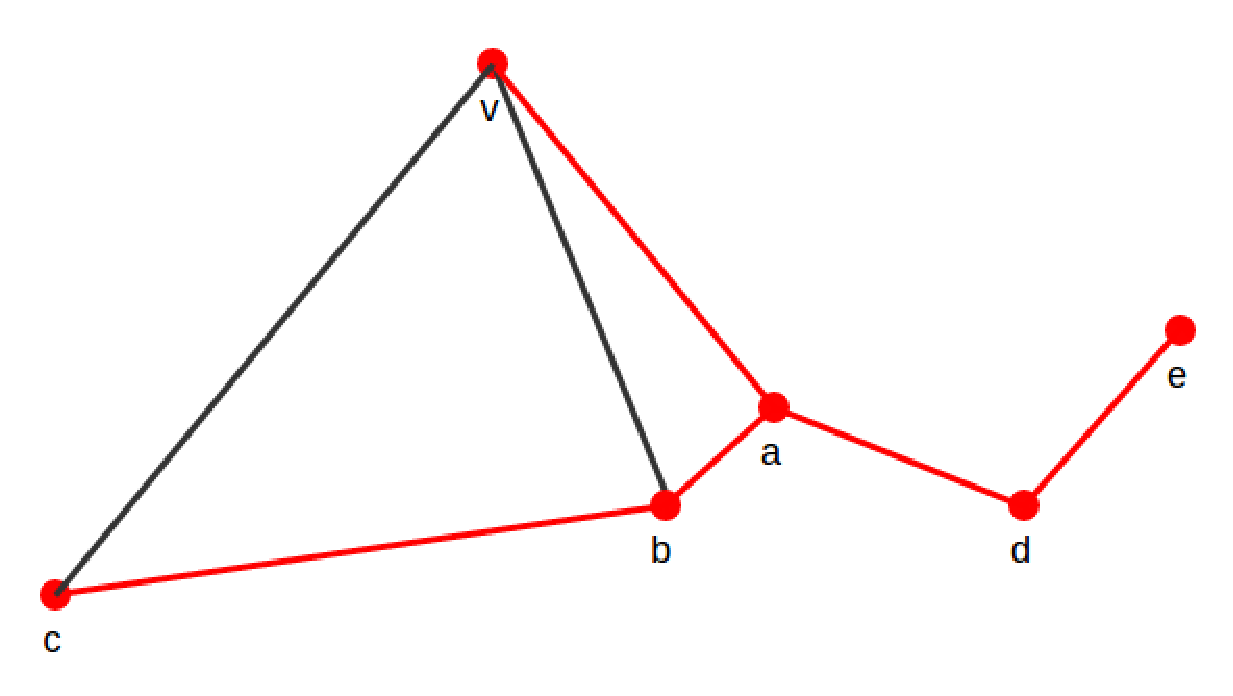
\includegraphics[scale=0.25]{figuras/capitulo2/dfs/dfs6.eps}
	\caption[Exemplo DFS etapa 6]{Exemplo DFS etapa 6 \cite{Cormen:2001}}
	\label{dfs6}
\end{figure}

Ao alcançar o vértice \textit{e}, não existem vértices não visitados, mesmo na volta no caminho. Portanto, o percurso realizado pelo \textit{DFS} pode ser observado na Figura \ref{dfs_percurso}, o qual é uma árvore.

\begin{figure}[!h]
	\centering
	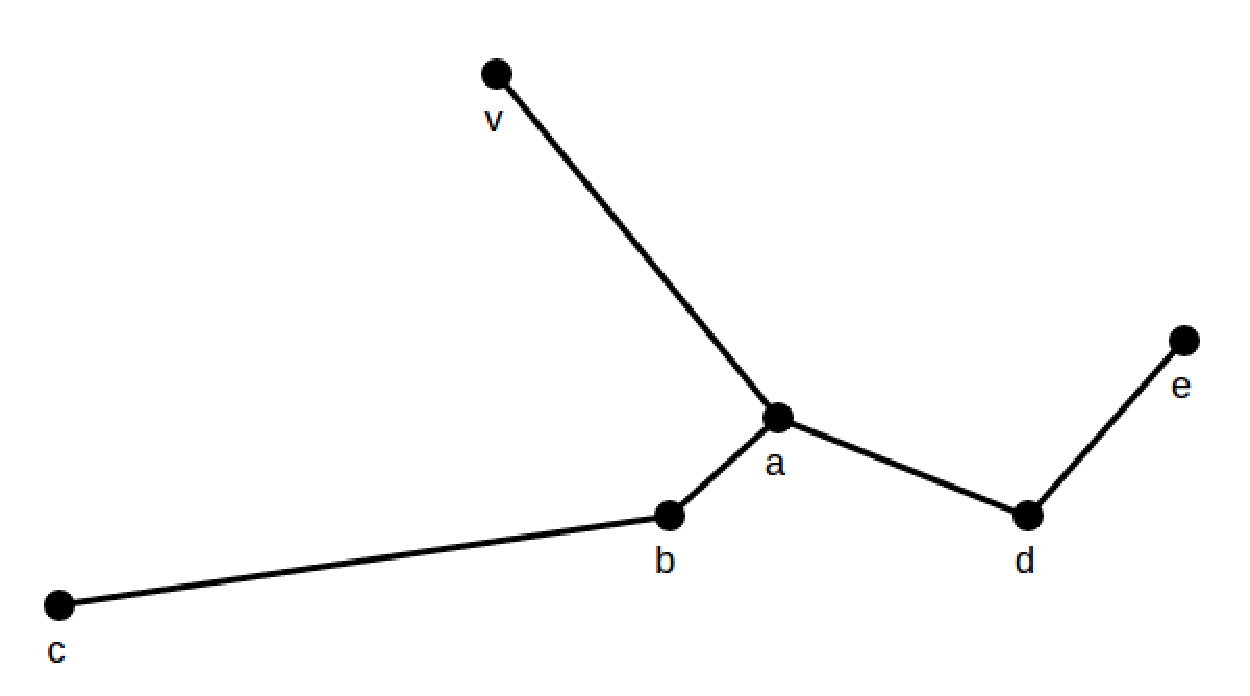
\includegraphics[scale=0.25]{figuras/capitulo2/dfs/dfs_percurso.eps}
	\caption[Percurso do DFS]{Percurso do DFS \cite{Cormen:2001}}
	\label{dfs_percurso}
\end{figure}

\section{Árvore Geradora Mínima}

Uma árvore geradora de um grafo G é uma árvore contendo todos os vértices de G e as arestas que são suficientes para transformar o grafo em uma árvore. Desse modo, uma árvore geradora de custo mínimo de um grafo G é um subgrafo conexo de G, uma árvore, contendo todos os vértices de G, de modo que a soma dos pesos das arestas no subgrafo seja mínima \cite{Rezende:2002}.

Existem dois principais algoritmos para árvores geradoras mínimas \cite{Bondy:2007}:

\subsection{Algoritmo de Prim}

A partir de um grafo \textit{G}, não dirigido e com pesos nas arestas. Escolhe-se um vértice \textit{v} qualquer de \textit{G}, em seguida é feito um corte em \textit{G}, ({\textit{v}}, \textit{G} $\backslash$ {\textit{v}}) com respeito a \textit{v}. Inicialmente tem-se \textit{T} = {\textit{v}}, onde \textit{T} ao final será a solução do algoritmo de Prim. A aresta de menor peso, \textit{e}, desse corte é escolhida, e esta aresta é incluída em \textit{T} (\textit{T} = \textit{T} $\cup$ {\textit{e}}), até que todos os vértices tenham sido cobertos, é feito um novo corte e a aresta de menor peso é incluída em T.

\subsection{Algoritmo de Kruskal}

Primeiramente, ordena-se as arestas de \textit{G}. Considera-se, então, cada vértice de \textit{G} como pertencendo a uma árvore em \textit{G}, ou seja, $\textit{v}_i \in \textit{T}_i , 1 \leq i \leq |\textit{V}|$. é verificado se a menor aresta de \textit{G} une dois vértices pertencentes a árvores diferentes. Se sim, as árvores são unidas e a operação é repetida. Se não, escolhe-se a próxima aresta da lista ordenada e a operação é repetida até que todas as subárvores de \textit{G} estejam unidas.

\chapter{Reutilização de Software}

\section{Padrão Abstract Factory}
\label{sec:padrao abstract factory}

A seguir, têm-se uma breve descrição do padrão ``\textit{Abstract Factory}'', como foi definido em \cite{Gamma:1995}.

Esse padrão fornece uma estrutura para criação de famílias de objetos relacionados sem a necessidade de definir suas classes concretas. A Figura \ref{abstract factory} apresenta o modelo do ``\textit{Abstract Factory}''.

\begin{figure}[!h]
	\centering
	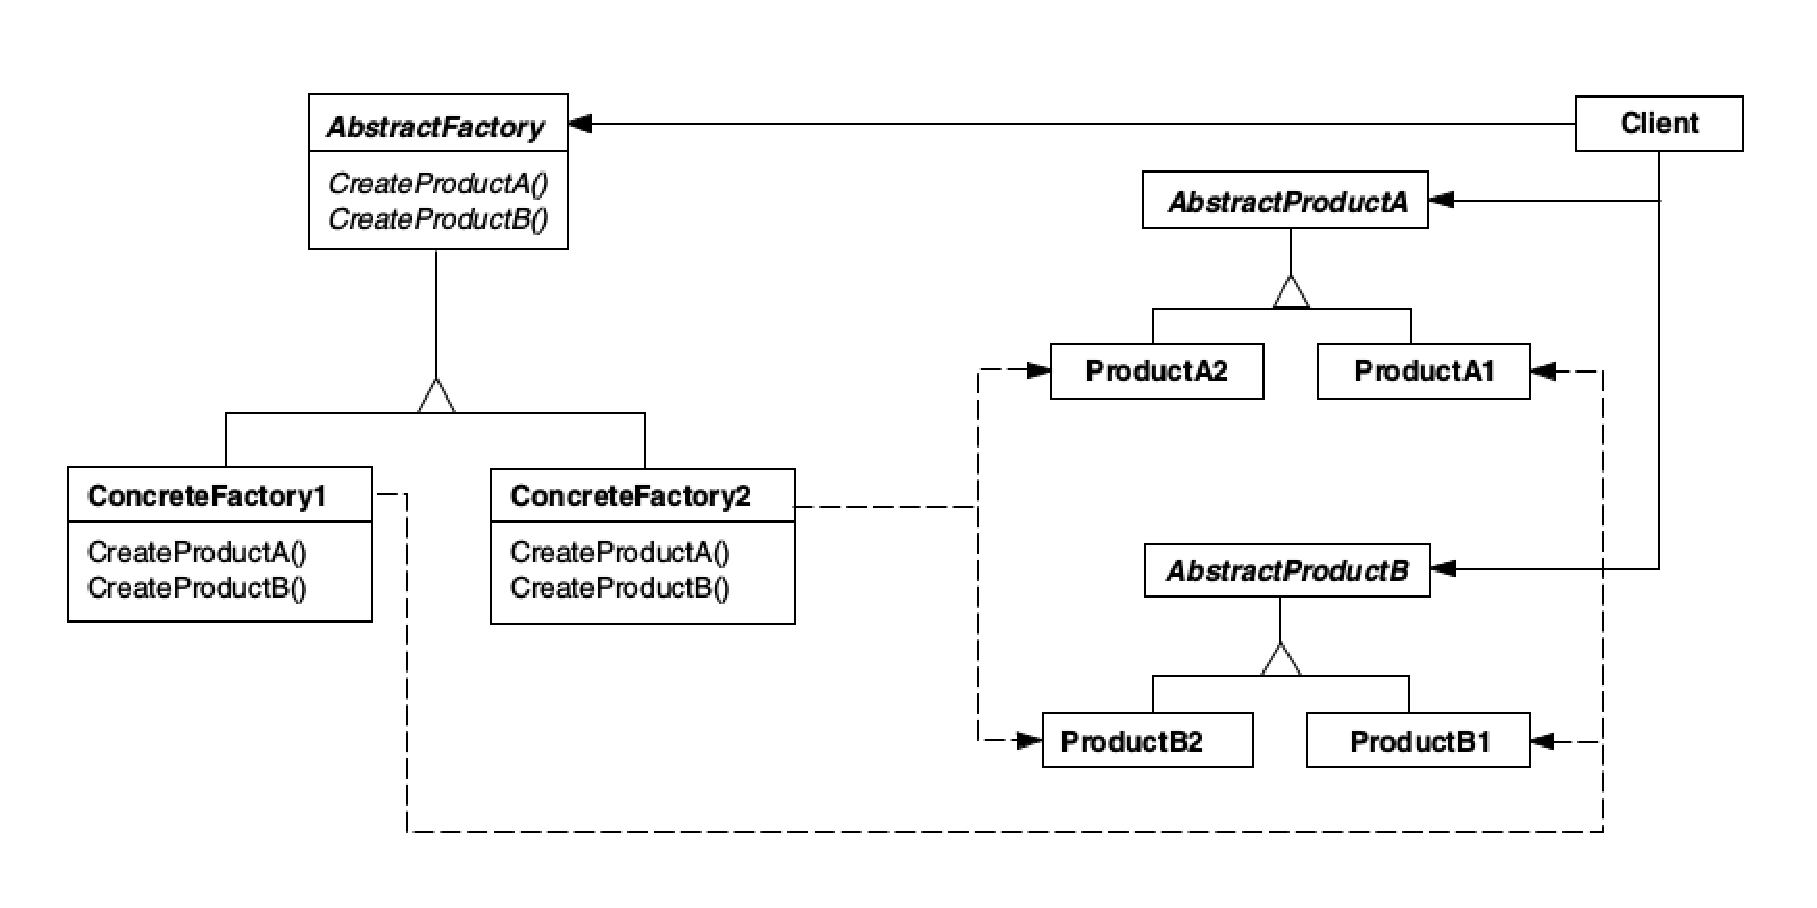
\includegraphics[scale=0.5]{figuras/capitulo2/abstract_factory.eps}
	\caption[Modelo genérico do Abstract Factory]{Modelo genérico do Abstract Factory \cite{Gamma:1995}}
	\label{abstract factory}
\end{figure}

O modelo da Figura apresenta cinco tipos de classes. ``\textit{Abstract Factory}'', ``\textit{Concrete Factory}'', ``\textit{Abstract Product}'', ``\textit{Product}'' e ``\textit{Client}''.

\begin{itemize}
	\item \textbf{\textit{Abstract Factory:}} Faz declarações de interfaces para criação de quaisquer produtos;
	\item \textbf{\textit{Concrete Factory:}} Essas classes já estão focadas no tipo de produtos que vão criar e implementam os métodos abstratos para essa criação;
	\item \textbf{\textit{Abstract Product:}} Classes abstratas que declaram interfaces para um determinado tipo de produto que deverá ser criado;
	\item \textbf{\textit{Product:}} Classes que representam o próprio produto que deverá ser criado, são as classes que são chamadas pelos métodos de criação presentes nas ``\textit{Concrete Factory}'';
	\item \textbf{\textit{Client:}} É a classe que representa quem irá fazer as chamadas aos métodos de criação. Não é necessário que conheça de fato as classes concretas de produto, pois apenas faz uso das interfaces declaradas em ``\textit{Abstract Factory}'' e ``\textit{Abstract Product}''; a primeira para criar os produtos, e a segunda para usá-los.
\end{itemize}

Este padrão oferece algumas vantagens e desvantagens que são apresentadas a seguir:

\begin{itemize}
	\item \textbf{Isolamento de classes concretas:} O cliente pode trabalhar com as criações dos produtos sem necessariamente conhecer as classes concretas que existem por traz, pois este trabalha apenas com as interfaces abstratas providas.
	\item \textbf{Fácil troca de famílias de produtos:} Basta trocar qual é a classe concreta que deverá ser usada que todo o comportamento dos produtos irá se alterar de acordo com essa classe. Isso pode ser feito facilmente no momento de instanciação da fábrica.
	\item \textbf{Harmonia entre produtos:} Como o padrão permite aos clientes trabalharem apenas com uma família por vez, fica fácil alcançar harmonia, pois todos os produtos da família estão de alguma forma relacionados.
	\item \textbf{Suporte a novos tipos de produtos é difícil:} Como a interface do ``\textit{Abstract Factory}'', no início, cria uma quantidade fixa de produtos para serem implementados, alterar isso fica difícil, pois é necessário mexer na classe principal e criar as subclasses concernentes.
\end{itemize}

A seguir será apresentada uma outra forma de reutilização de software. Os serviços que tem sido usados cada vez mais em projetos de desenvolvimento.

\end{apendicesenv}
